\documentclass[12pt,a4paper]{article}

\usepackage[utf8]{inputenc}
\usepackage[T1]{fontenc}
\usepackage[brazilian]{babel}
\usepackage{lmodern}
\usepackage{geometry}
\usepackage{array}
\usepackage{tabularx}
\usepackage{booktabs}
\usepackage{enumitem}
\usepackage{graphicx}
\usepackage{float}
\usepackage{xcolor}
\usepackage{hyperref}

\geometry{top=2.5cm,bottom=2.5cm,left=2.8cm,right=2.8cm}
\graphicspath{{telas/}}
\hypersetup{
  colorlinks=true,
  linkcolor=black,
  urlcolor=blue
}
\setlist[itemize]{leftmargin=*, itemsep=3pt, topsep=4pt}
\renewcommand{\arraystretch}{1.18}

\title{\textbf{Relatório de Alterações}\\Interface, Responsividade e Acessibilidade}
\author{Uender Barbosa de Souza}
\date{}

\begin{document}

\maketitle

\section{Visão Geral}

Foram realizadas melhorias na interface pública, na chave dicotômica e no painel administrativo do sistema. O objetivo foi tornar a navegação mais clara, melhorar a apresentação em telas pequenas e corrigir pontos de acessibilidade observados durante os testes.

As alterações mantiveram a estrutura atual do projeto e o funcionamento da API pública.

\section{Arquivos Criados}

\begin{tabularx}{\textwidth}{>{\raggedright\arraybackslash\footnotesize}p{0.45\textwidth} X}
\toprule
\normalfont\textbf{arquivo} & \textbf{descrição} \\
\midrule
\path{assets/css/ui-base.css} & estilos compartilhados de foco visível e redução de movimento \\
\path{assets/css/admin-responsive.css} & comportamento responsivo das telas administrativas \\
\path{assets/js/admin-layout.js} & controle do menu mobile e adaptação das tabelas do admin \\
\path{docs/RELATORIO_IMPLEMENTACAO_UI_ACESSIBILIDADE.md} & descrição dos blocos implementados e testes realizados \\
\path{docs/telas/} & capturas das telas verificadas durante os testes \\
\bottomrule
\end{tabularx}

\section{Área Pública}

\subsection{Página Principal (\texttt{index.php})}

\begin{itemize}
  \item Foi incluída uma orientação inicial para informar ao aluno como iniciar a identificação.
  \item Os botões dos cards foram renomeados para \texttt{Ver características} e \texttt{Iniciar identificação}.
  \item O acesso à área administrativa foi ajustado para não sobrepor o título em telas de celular.
  \item O botão de ajuda foi removido, pois ainda não possuía função implementada.
  \item Registros sem imagem agora exibem o texto \texttt{Imagem não cadastrada} em um componente visual discreto.
\end{itemize}

\subsection{Modal de Detalhes}

\begin{itemize}
  \item O modal recebeu estrutura adequada de diálogo, com título associado.
  \item O fechamento pode ser feito pelo botão, pelo fundo da tela ou pela tecla \texttt{Escape}.
  \item Ao abrir o modal, o foco é direcionado para o conteúdo.
  \item Ao fechar, o foco retorna ao botão que abriu os detalhes.
\end{itemize}

\section{Chave Dicotômica (\texttt{chave.php})}

\subsection{Navegação}

\begin{itemize}
  \item A tela passou a exibir progresso textual junto com a barra de progresso.
  \item Foi adicionado o painel \texttt{Histórico da identificação}, que mostra as escolhas feitas durante a identificação atual.
  \item Foi incluído o botão \texttt{Voltar ao passo anterior}, respeitando o caminho realmente percorrido pelo aluno.
  \item Ao selecionar uma alternativa, as duas opções ficam bloqueadas durante a transição para evitar cliques repetidos.
  \item O histórico é apagado ao refazer a identificação ou recarregar a página.
\end{itemize}

\subsection{Apresentação}

\begin{itemize}
  \item O texto \texttt{Specimen Match} foi substituído por \texttt{Chave dicotômica}.
  \item As alternativas foram reorganizadas para ocupar menos espaço no desktop.
  \item Em celulares, as opções passaram a ser apresentadas em cards compactos, com imagem, descrição e botão no mesmo bloco.
  \item Imagens ausentes passaram a usar o mesmo padrão visual adotado na página principal.
\end{itemize}

\subsection{Acessibilidade}

\begin{itemize}
  \item A barra de progresso utiliza \texttt{role="progressbar"} e atributos ARIA atualizados a cada passo.
  \item Foi adicionada uma região de aviso para informar passo atual e família identificada.
  \item Os botões possuem nomes diferentes para cada alternativa, incluindo a descrição da opção.
  \item O foco é direcionado para a pergunta ao avançar ou voltar e para o resultado ao concluir.
  \item Os controles principais possuem área de clique adequada para uso em telas sensíveis ao toque.
\end{itemize}

\section{Área Administrativa}

\subsection{Autenticação}

\begin{itemize}
  \item O redirecionamento de páginas protegidas foi corrigido para funcionar no caminho atual do projeto.
  \item O formulário de login recebeu rótulos associados aos campos e configuração de preenchimento automático.
  \item Foi removido o processamento duplicado do login na mesma página.
\end{itemize}

\subsection{Layout Responsivo}

\begin{itemize}
  \item A barra lateral continua fixa no desktop.
  \item Em telas menores, a navegação passou a funcionar como menu lateral recolhível.
  \item O menu possui botão de abertura, sobreposição de fundo e fechamento pela tecla \texttt{Escape}.
  \item O foco retorna ao botão \texttt{Menu} depois do fechamento por teclado.
  \item As tabelas passam a ser exibidas como cards rotulados em celulares.
  \item Formulários, filtros e seletores passam a ocupar uma única coluna em telas pequenas.
\end{itemize}

As telas adaptadas foram:

\begin{itemize}
  \item Dashboard;
  \item Ordens;
  \item Famílias;
  \item Chaves Dicotômicas;
  \item Administradores.
\end{itemize}

\subsection{Imagens Pendentes}

\begin{itemize}
  \item O dashboard agora apresenta contadores de itens sem imagem cadastrada.
  \item As listagens de ordens e famílias exibem badge \texttt{Sem imagem}.
  \item O editor de chaves identifica alternativas sem imagem.
  \item Os formulários apresentam um estado vazio para pré-visualização quando ainda não existe imagem cadastrada.
\end{itemize}

Contagens verificadas no banco durante os testes:

\begin{center}
\begin{tabular}{lr}
\toprule
\textbf{item} & \textbf{quantidade sem imagem} \\
\midrule
Ordens & 12 \\
Famílias & 69 \\
Alternativas da chave & 8 \\
\bottomrule
\end{tabular}
\end{center}

\section{Arquivos Alterados}

\begin{tabularx}{\textwidth}{>{\raggedright\arraybackslash\footnotesize}p{0.35\textwidth} X}
\toprule
\normalfont\textbf{arquivo} & \textbf{alteração principal} \\
\midrule
\path{index.php} & orientação inicial, modal acessível e novos estados sem imagem \\
\path{chave.php} & progresso acessível, histórico, retorno e bloqueio de seleção \\
\path{includes/db.php} & correção do redirecionamento administrativo \\
\path{admin/login.php} & melhoria do formulário de acesso \\
\path{admin/index.php} & indicadores de imagens pendentes e suporte ao layout responsivo \\
\path{admin/ordens.php} & badges, preview e responsividade \\
\path{admin/familias.php} & badges, preview e responsividade \\
\path{admin/chaves.php} & indicadores das alternativas, preview e responsividade \\
\path{admin/admins.php} & responsividade das tabelas e formulários \\
\path{assets/css/site-home.css} & acabamento e adaptação da página principal \\
\path{assets/css/site-chave.css} & layout e responsividade da chave \\
\bottomrule
\end{tabularx}

\section{Compatibilidade}

\begin{itemize}
  \item A API pública em \texttt{api.php} manteve as mesmas actions e o mesmo formato de resposta.
  \item O histórico da chave é mantido somente na memória da página e não é gravado no banco.
  \item Não foram adicionadas imagens de conteúdo; os registros pendentes continuam disponíveis para preenchimento posterior.
  \item O fluxo de upload existente para ordens, famílias e alternativas foi preservado.
\end{itemize}

\section{Testes Realizados}

\begin{itemize}
  \item Verificação de sintaxe dos arquivos PHP alterados.
  \item Acesso à página administrativa protegida sem sessão e validação do redirecionamento para o login.
  \item Login, acesso ao dashboard e logout.
  \item Abertura e fechamento do modal da página principal.
  \item Verificação visual da página principal em desktop e celular.
  \item Percurso completo na chave \emph{Hemiptera-Auchenorrhyncha}, com conclusão em \emph{Cicadellidae}.
  \item Testes de voltar passo, refazer identificação e recarregar a página sem manter histórico.
  \item Verificação da chave em desktop e celular, sem rolagem horizontal.
  \item Verificação das telas administrativas em desktop, tablet e celular.
  \item Teste do menu administrativo mobile por botão, fundo da tela e tecla \texttt{Escape}.
  \item Comparação dos indicadores de imagens pendentes com consultas diretas ao banco.
  \item Verificação de erros no navegador durante os fluxos testados.
\end{itemize}

\clearpage
\section{Evidências Visuais}

As capturas realizadas durante os testes estão na pasta \texttt{docs/telas/}.

\subsection{Página Principal}

\begin{figure}[H]
  \centering
  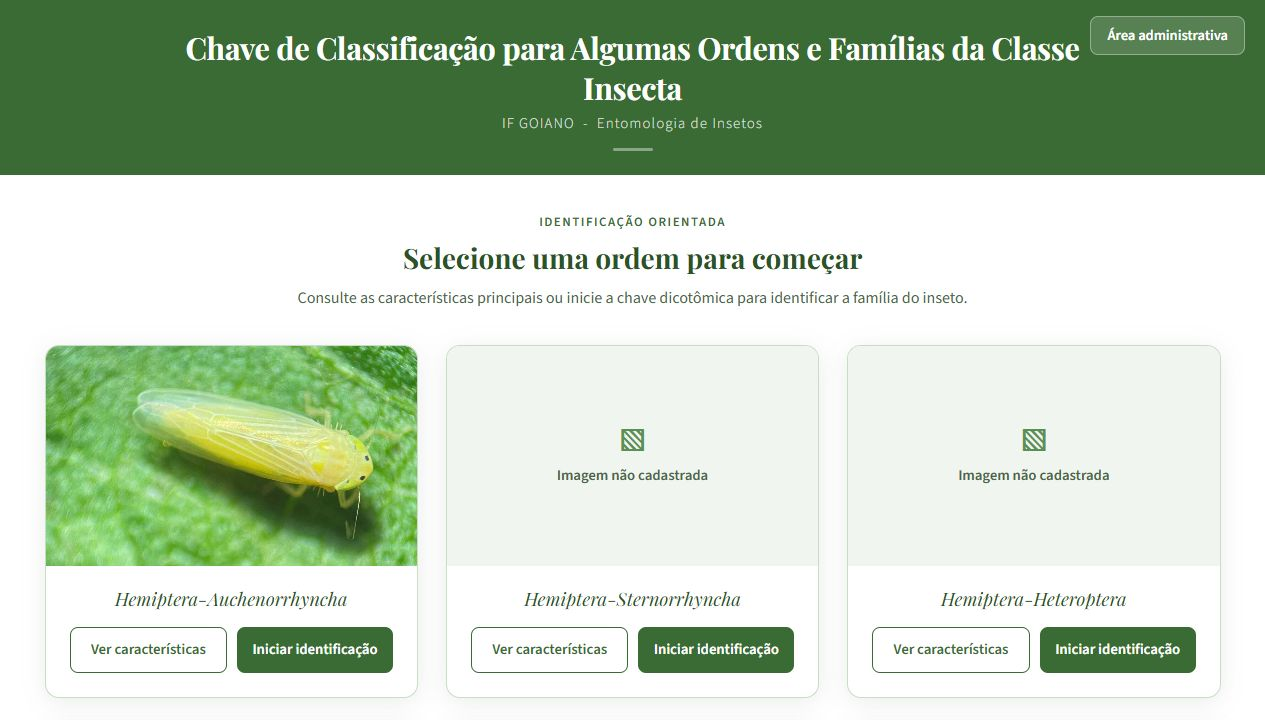
\includegraphics[width=\textwidth]{home-desktop.png}
  \caption{Página principal em computador.}
\end{figure}

\begin{figure}[H]
  \centering
  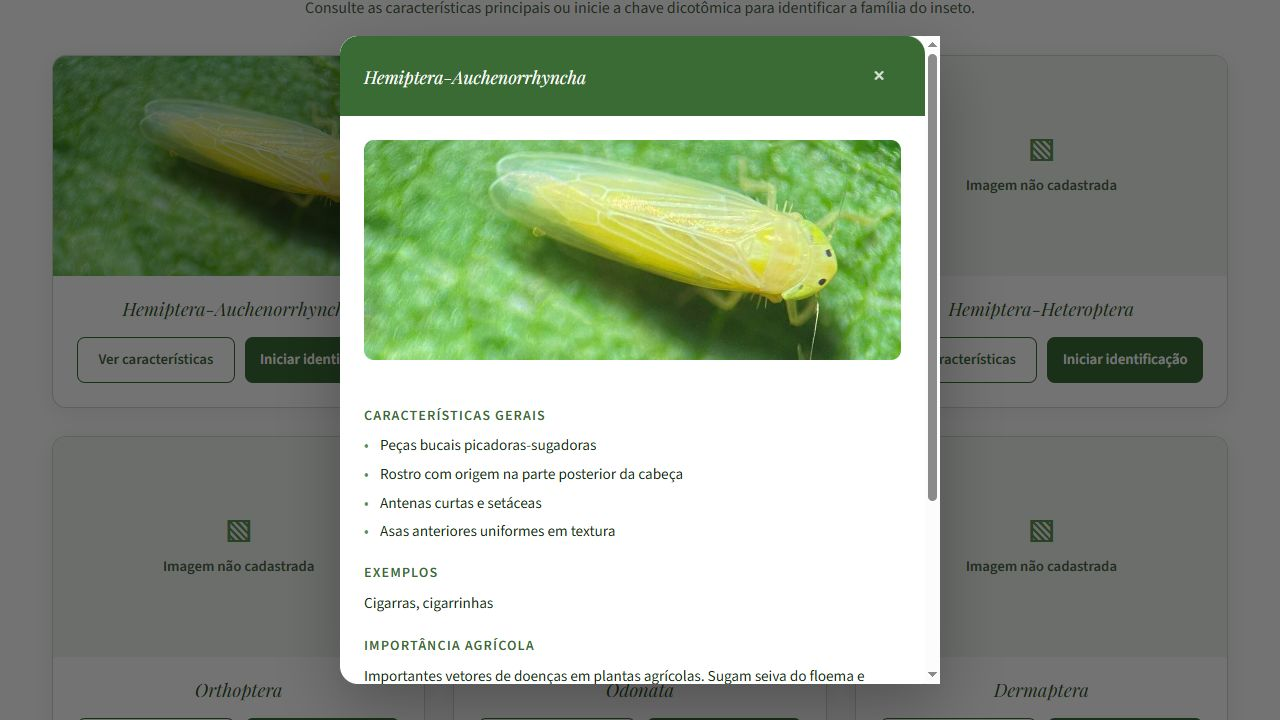
\includegraphics[width=0.88\textwidth]{home-modal-desktop.png}
  \caption{Modal de detalhes da ordem na versão para computador.}
\end{figure}

\begin{figure}[H]
  \centering
  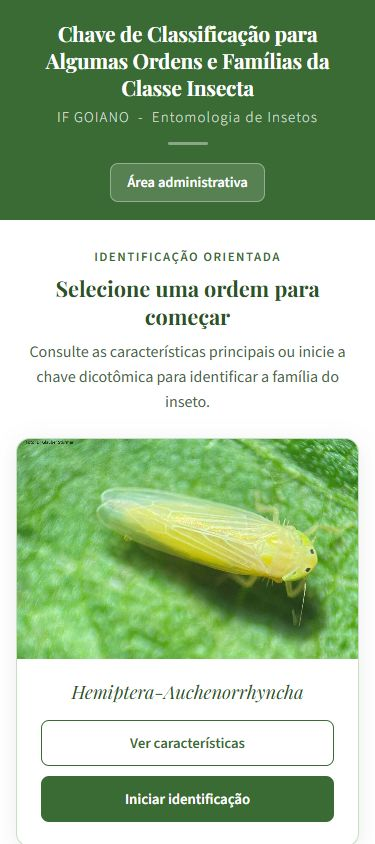
\includegraphics[height=0.67\textheight]{home-mobile.png}
  \caption{Página principal na versão para celular.}
\end{figure}

\clearpage
\subsection{Chave Dicotômica}

\begin{figure}[H]
  \centering
  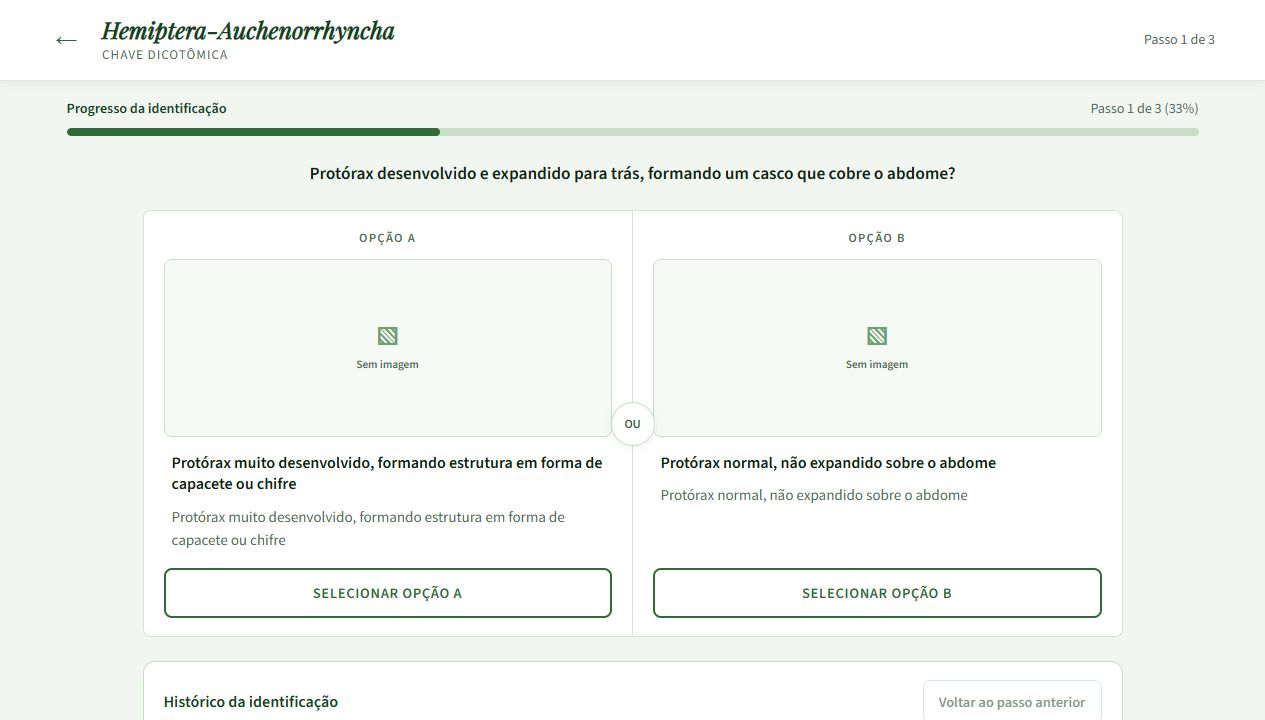
\includegraphics[width=\textwidth]{chave-desktop.png}
  \caption{Passo da chave dicotômica na versão para computador.}
\end{figure}

\begin{figure}[H]
  \centering
  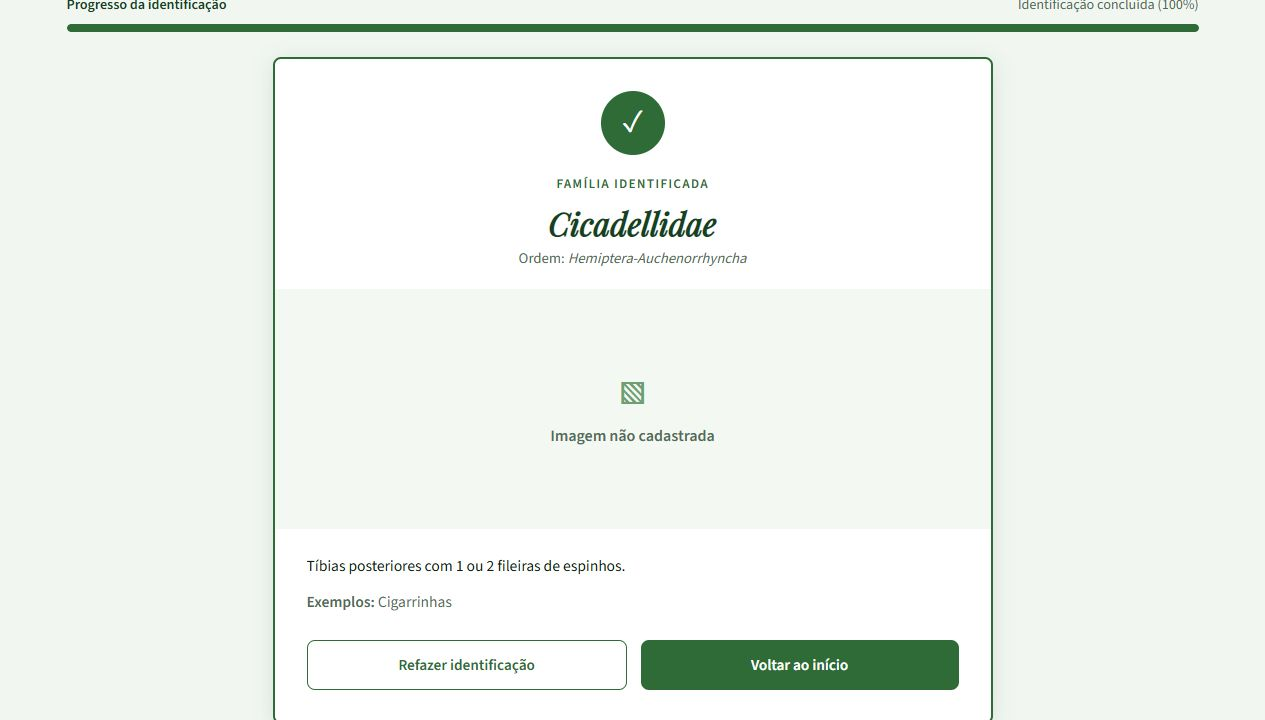
\includegraphics[width=0.8\textwidth]{chave-resultado-desktop.png}
  \caption{Resultado obtido após concluir a identificação.}
\end{figure}

\begin{figure}[H]
  \centering
  \begin{minipage}{0.47\textwidth}
    \centering
    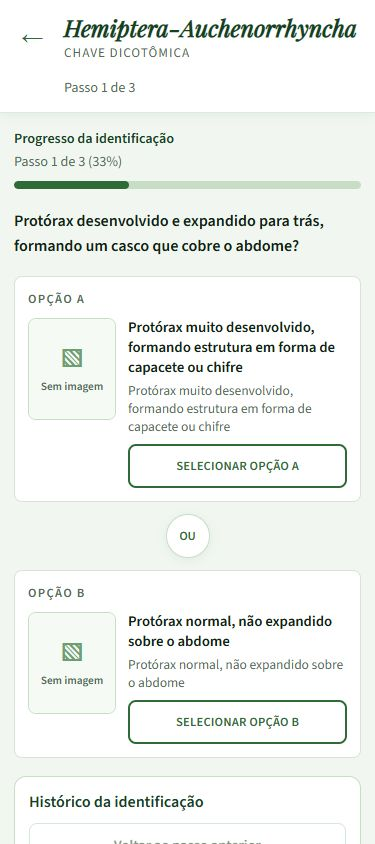
\includegraphics[width=\textwidth]{chave-mobile.png}
    \caption{Chave em celular.}
  \end{minipage}
  \hfill
  \begin{minipage}{0.47\textwidth}
    \centering
    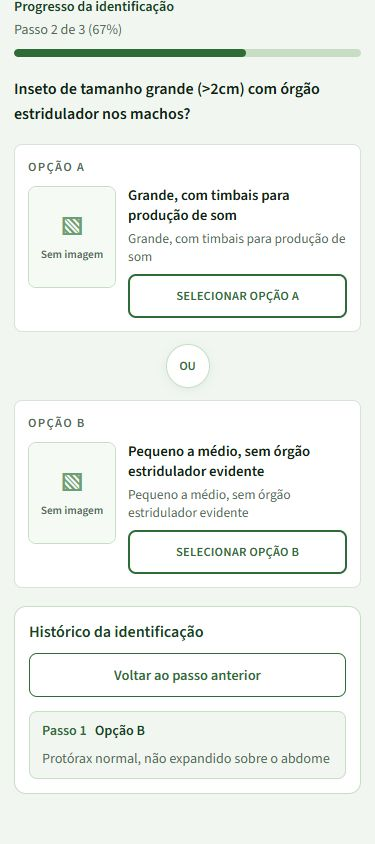
\includegraphics[width=\textwidth]{chave-mobile-historico.png}
    \caption{Histórico das escolhas no celular.}
  \end{minipage}
\end{figure}

\clearpage
\subsection{Área Administrativa}

\begin{figure}[H]
  \centering
  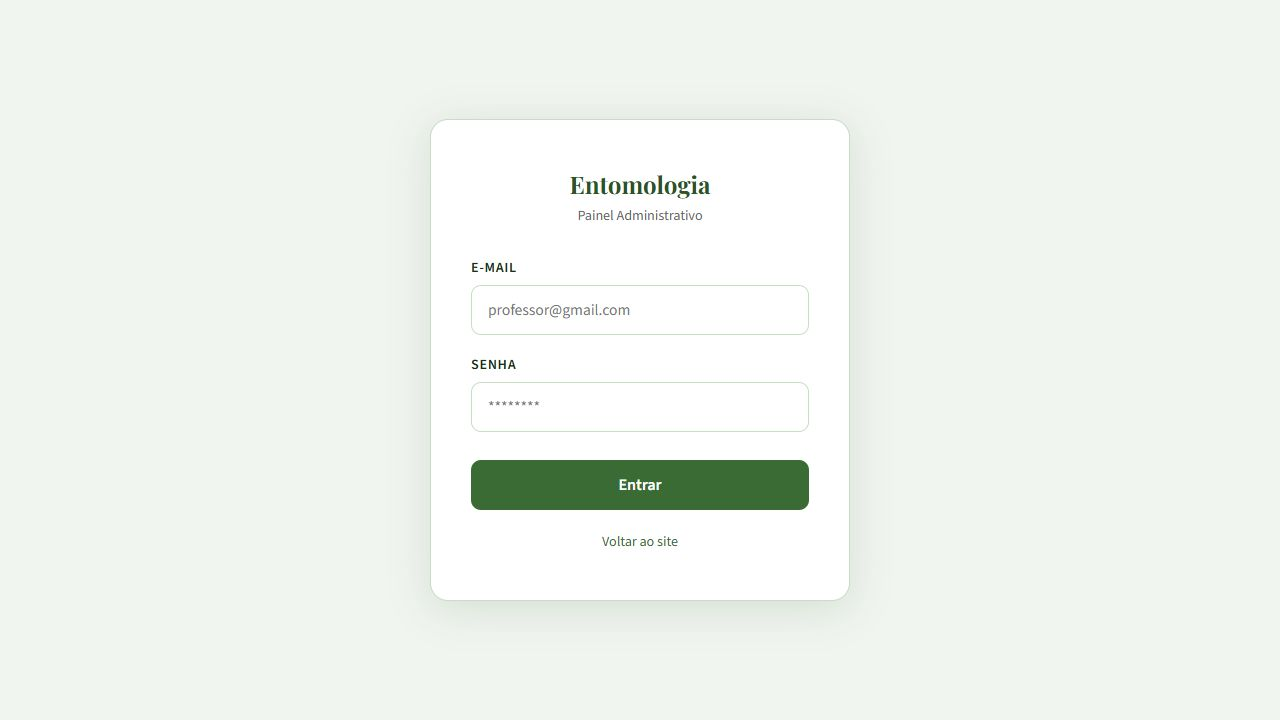
\includegraphics[width=0.86\textwidth]{admin-login-desktop.png}
  \caption{Tela de login administrativo.}
\end{figure}

\begin{figure}[H]
  \centering
  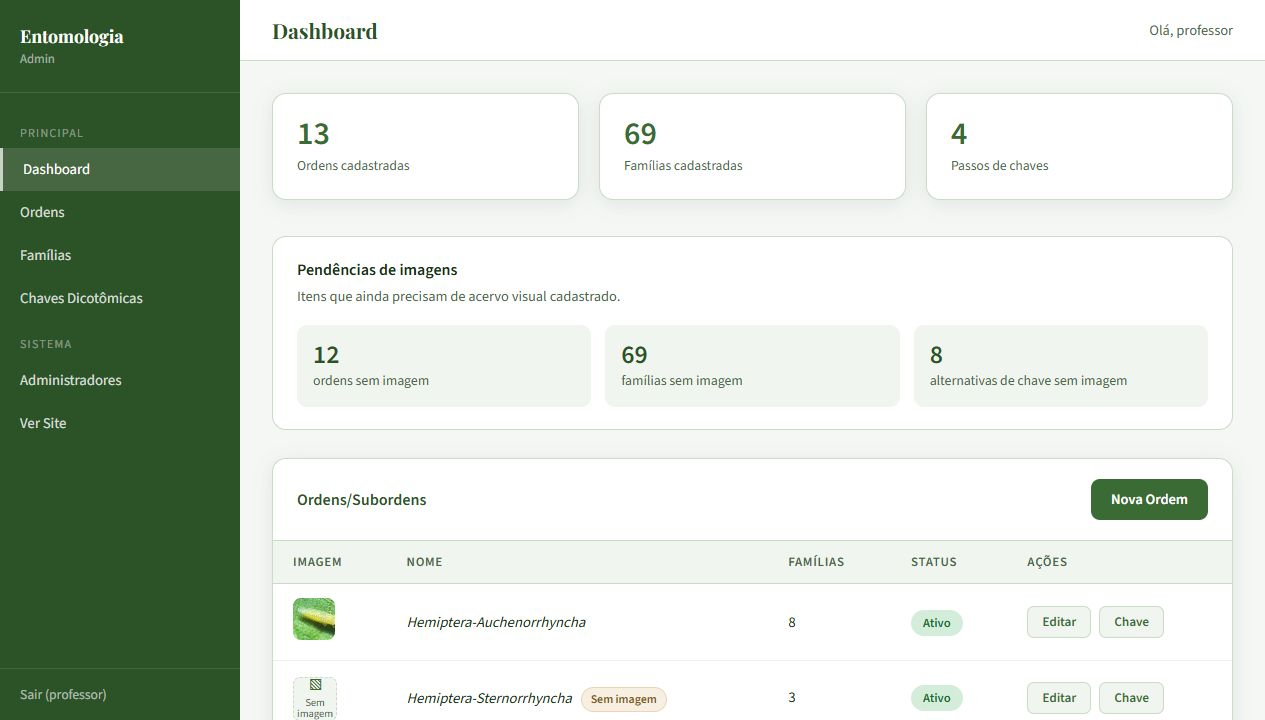
\includegraphics[width=\textwidth]{admin-dashboard-desktop.png}
  \caption{Dashboard com indicadores de imagens pendentes.}
\end{figure}

\begin{figure}[H]
  \centering
  \begin{minipage}{0.47\textwidth}
    \centering
    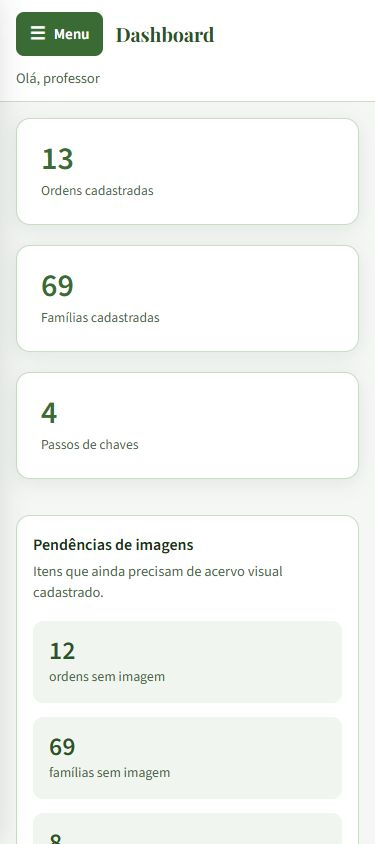
\includegraphics[width=\textwidth]{admin-dashboard-mobile.png}
    \caption{Dashboard no celular.}
  \end{minipage}
  \hfill
  \begin{minipage}{0.47\textwidth}
    \centering
    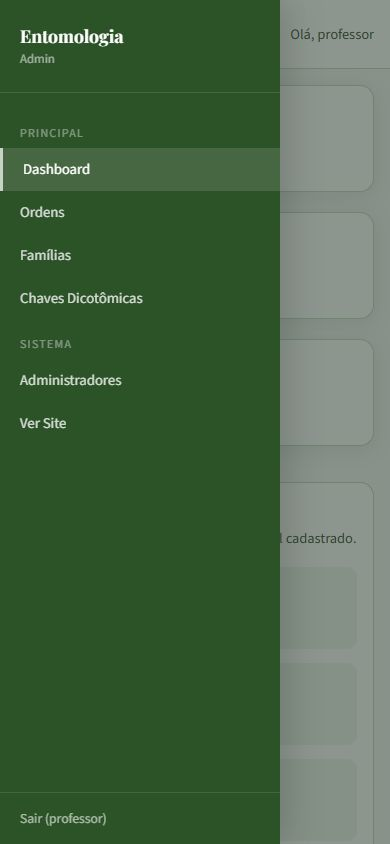
\includegraphics[width=\textwidth]{admin-drawer-mobile.png}
    \caption{Menu lateral aberto no celular.}
  \end{minipage}
\end{figure}

\begin{figure}[H]
  \centering
  \begin{minipage}{0.47\textwidth}
    \centering
    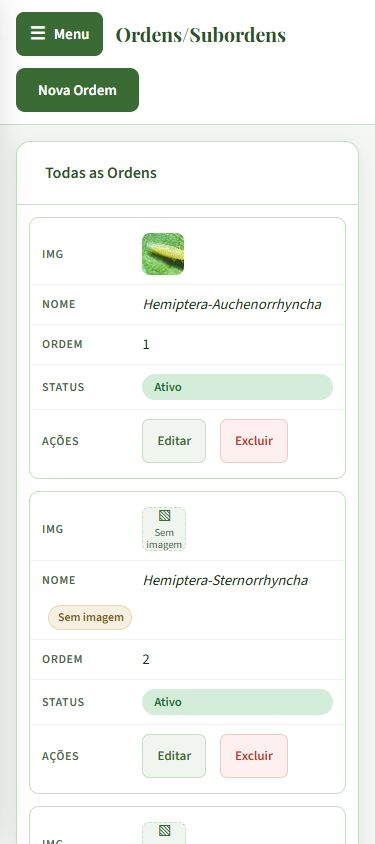
\includegraphics[width=\textwidth]{admin-ordens-mobile.png}
    \caption{Listagem de ordens no celular.}
  \end{minipage}
  \hfill
  \begin{minipage}{0.47\textwidth}
    \centering
    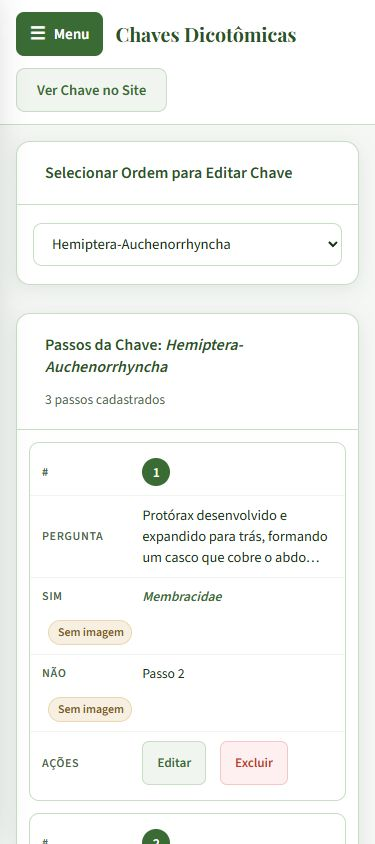
\includegraphics[width=\textwidth]{admin-chaves-mobile.png}
    \caption{Editor de chaves no celular.}
  \end{minipage}
\end{figure}

\clearpage
\section{Mapeamento do Sistema com Graphify}

Foi gerado um grafo do projeto utilizando a ferramenta Graphify, que pode ser acessado na pasta \texttt{graphify-out}. Esse grafo serve para mapear as dependências, as comunidades lógicas e o fluxo de dados entre os arquivos e componentes do sistema, facilitando a compreensão visual da arquitetura do projeto.

\begin{figure}[H]
  \centering
  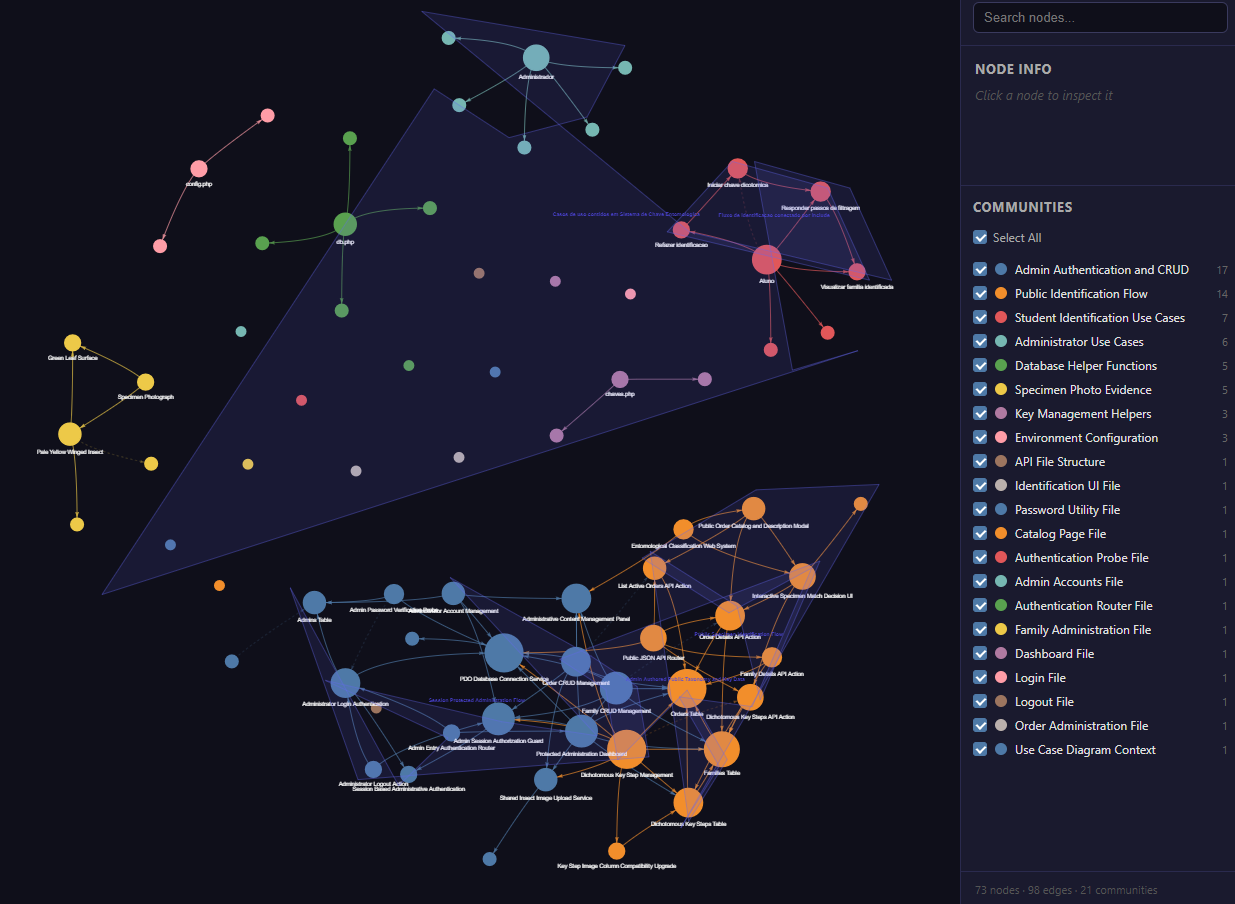
\includegraphics[width=\textwidth]{grafo.png}
  \caption{Grafo gerado pelo Graphify.}
\end{figure}

\section{Próximas Melhorias}

\subsection{Evitar hard delete em dados principais}

Ordens e famílias podem ser excluídas definitivamente, com cascata. Sugestões:

\begin{itemize}
  \item Preferir inativação ou soft delete para dados usados em contexto acadêmico.
  \item Exibir impacto antes de excluir, como quantidade de famílias e passos afetados.
  \item Manter trilha de auditoria para ações administrativas.
  \item Impedir exclusão acidental de dados usados em chaves publicadas.
\end{itemize}

\end{document}
